\documentclass[a4paper,11pt]{article}
\usepackage[T1]{fontenc}
\usepackage[utf8]{inputenc}
\usepackage{lmodern}
\usepackage[english]{babel}
\usepackage{hyperref}
\usepackage{wrapfig}
\usepackage{graphicx}
\usepackage{mathtools}

\usepackage{amsmath}
\usepackage{amssymb}
\usepackage{tabularx}
\usepackage{bm}
\usepackage{tikz}


% tizk options
\usetikzlibrary{arrows}
\usetikzlibrary{calc}
\usetikzlibrary{positioning}
\usetikzlibrary{decorations, decorations.pathmorphing,decorations.pathreplacing}

\tikzstyle{block} = [draw,rectangle,thick,minimum height=2em,minimum width=2em]
\tikzstyle{connector} = [->,thick]
\tikzstyle{merge} = [draw, circle, thick,minimum height=2em,minimum width=2em]

\hypersetup{
  colorlinks   = true, %Colours links instead of ugly boxes
  urlcolor     = blue, %Colour for external hyperlinks
  linkcolor    = black, %Colour of internal links
  citecolor   = black %Colour of citations
}

\newtheorem{assumption}{Assumption}



\title{Claptrap simulation and control.}
\author{Matthieu Vigne}

\begin{document}
\maketitle
\tableofcontents

\section{Introduction}

In order to design controllers for a complex system such as Claptrap, knowing the equation of motion and being able to simulate them is crucial. This document covers both of these aspects. In a first part, it presents the kinematics of the system, and how to simulate it easily, assuming perfect, non-slipping wheel-ground contact, using a dynamics library like \emph{pinocchio}. In a second (upcomming) part, an analysis of these equations is performed, in order to design and test plausible controllers.

\section{Claptrap Kinematics and Simulation}

\subsection{System overview}

The dynamics of Claptrap are just a particular case of rigid body dynamics. Luckily, this is a very well studied problem, with efficient state-of-art algorithms available to solve this. In particular, Roy Featherstone's "Rigid Body Dynamics" is a well-known reference in the field ; the algorithms presented therein (and others) are all efficiently implemented in the open-source library \emph{pinocchio}, that we will be using for doing the simulation.

All that we need to apply these algorithms is to give them a description of the kinematics (i.e. geometry) of the system, and the relevant dynamic parameters (mass and inertia of each rigid body constituting the system) : all this can be done using a URDF model.

\begin{figure}
	\centering
	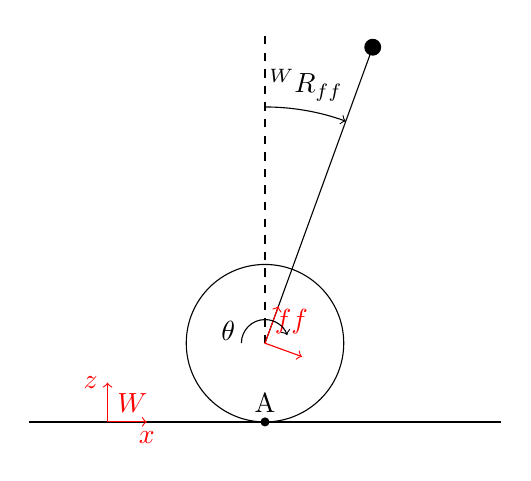
\begin{tikzpicture}
	\draw[thick] (-3, 0) -- (3,0);
	
	\draw (0, 1) circle(1);
	
	\draw[dashed] (0, 1) -- (0, 5);
	\begin{scope}[rotate around={-20:(0,1)}]
		\draw (0, 1) -- (0, 5);
		\filldraw (0,5) circle(0.1);
		\draw[<->, red] (0, 1.5) --++ (0, -0.5)node[above right] {$ff$} --++ (0.5,0);
	\end{scope}
	
	\draw[->] (0, 4) arc(90:70:3) node[pos=0.5, above] {${}^W R_{ff}$};
	
	\draw[->] (-0.3, 1) arc(180:20:0.3) node[pos=0.2, left] {$\theta$};
	
	\draw[<->, red] (-2, 0.5) --++ (0, -0.5)node[left, pos=0] {$z$} node[above right] {$W$} --++ (0.5,0) node[below] {$x$};
	
	
	\filldraw (0,0) circle(0.05) node[above] {A};
	\end{tikzpicture}
	\caption{Claptrap kinematics.}
	\label{fModel}
\end{figure}

For the sake of illustration, we will consider a 2D version of Claptrap without arms: indeed, the only difficulty comes from ground contact and freeflyer consideration ; adding internal degrees of freedom is not a problem at all. Then, Claptrap reduces to a simple pendulum on wheel system, as depicted in Figure~\ref{fModel}.

Let $\theta$ be the angle of the wheel with respect to the bar. Note that this is a relative angle, and not the angle of the bar with respect to the ground. Obviously this variable is not enough to characterize the motion of the system: being a mobile base system, six extra degrees of freedom (three in rotation, three in translation) characterize its position is space. The freeflyer can be seen as representing the pose of any point in the system: for simplicity, we will take here the center of the wheel as origin, with orientation matching the upper link bar: this is depicted as the $ff$ (freeflyer) frame in Figure~\ref{fModel}

We call $\bm q_ff$ the coordinates of the freeflyer. While only six degrees of freedom are present, in practice a rotation is represented in pinocchio using a quaternion: thus $\bm q_ff$ is a vector of dimension 7 ; its derivative however, $\bm v_{ff}$, needs only to contain six components. In detail (but this is not really important), these vectors write:

\begin{equation}
	\bm q_{ff} \triangleq \begin{pmatrix} {}^W p_{ff} \\ {}^W q_{ff} \end{pmatrix} \qquad
	\bm v_{ff} \triangleq \begin{pmatrix} {}^{ff} q_W {}^W \dot{p}_{ff} \\ \bm \omega_{ff} \end{pmatrix} 
\end{equation} 

where $\bm \omega_ff$ is the angular velocity associated to ${}^W R_{ff}$, i.e. ${}^W \dot{R}_{ff} = {}^W R_{ff} [\bm \omega_{ff}]_\times$ with $[.]_\times$ the skew-symmetric (cross product) operator.

\medskip

The generalized coordinates describing this them are simply obtained by concatenating the freeflyer with the internal joints. Note that in practice, the internal joints structure is given by the URDF, and the freeflyer is added when loading the model in \emph{pinocchio}: this is because these joints are slightly different in nature, the URDF means to characterized kinematic relationships inside a system, and the freeflyer encodes the relationship with the outside. In our example, we simply have


\begin{equation}
\bm q \triangleq \begin{pmatrix} \bm q_{ff} \\ \theta \end{pmatrix} \qquad
\bm v \triangleq \begin{pmatrix} \bm v_{ff} \\ \dot{\theta} \end{pmatrix}
\end{equation} 

\subsection{Implementing ground contact}

Lagrange's laws of motion tell us that the inverse dynamics of such a system writes

\begin{equation}
	H(\bm q) \dot{\bm v} + C(\bm q, \bm v) \bm v + \bm g(\bm q) = \bm f_{ext}
	\label{eqInverseDynamics}
\end{equation} 

where $H$ is the joint-space inertia matrix, $C$ the matrix representing Coriolis and centrifugal forces, $\bm g$ gravity, and $\bm F_{ext}$ the vector of external forces. These forces obviously include motor torques, but also ground forces that we need to consider here.

To represent ground contact, we make the following assumption:

\begin{assumption}
	The contact between the ground and the wheel is assumed to be punctual, happening at point $A$. Furthermore, we assume that the wheel does not slip on the ground. Finally, we only consider flat ground.
\end{assumption}

Ideal contact (i.e. no slippage at point $A$) implies that the velocity of point $A$ is zero. The position of point $A$ in turn is function of $\bm q$: thus, this constraint takes the generic form $\bm g(\bm q) = 0$. Let $J(\bm q)$ be the Jacobian of $\bm g$. This Jacobian appears in two important places:

 - first, it enables us to rewrite the non-linear constraint on $\bm q$ as a linear constraint on its derivative, $J(\bm q) \bm v = 0$, and then on its second derivative:
 
 \begin{equation}
 J(\bm q) \dot{\bm v} + \dot{J}(\bm q, \bm v) \bm v = 0
 \label{eqConstraint}
 \end{equation} 
 
 
 - second, its transpose links the ground reaction force to the vector of generalized forces $\bm f_{ext}$ in \eqref{eqInverseDynamics}. More specifically, $\bm f_{ext}$ is the sum of two effects: the motor torque $\bm tau$ applied on the joints, and the ground reaction force $\bm f_g$ (a vector in the Cartesian space) projected onto the joints using $J^T(\bm q)$:
 
 \begin{equation}
 \bm f_{ext} \triangleq J^T(\bm q) \bm f_g + \bm \tau
 \label{eqForce}
 \end{equation}
 
 
Then, using \eqref{eqInverseDynamics}, \eqref{eqConstraint} and \eqref{eqForce}, the constraint equation of dynamics writes:

\begin{equation}
\begin{aligned}
H(\bm q) \dot{\bm v} + C(\bm q, \bm v) \bm v + \bm g(\bm q) &= J^T(\bm q) \bm f_g + \bm \tau \\
J(\bm q) \dot{\bm v} + \dot{J}(\bm q, \bm v) \bm v &= 0
\end{aligned}
\label{eqInverseDynamicsConstaint}
\end{equation} 

This is a coupled system of equations of unknown $\dot{\bm v}$ and $\bm f_g$ (the state and input torque $\bm q$, $\bm v$, $\bm \tau$ being given). 

This system is easily solvable, as it is in fact linear:

\begin{equation}
\begin{pmatrix} H(\bm q) & J^T(\bm q) \\ J(\bm q) & 0 \end{pmatrix} \begin{pmatrix} \dot{\bm v} \\ \bm f_g \end{pmatrix} = \begin{pmatrix} \bm \tau - C(\bm q, \bm v) \bm v - \bm g(\bm q) \\ -\dot{J}(\bm q, \bm v) \bm v \end{pmatrix}
\label{eqID}
\end{equation} 

and the first matrix is invertible, granted that $J(\bm q)$ is full-ranked - in other words, that the constraints are linearly independent. This is the case in practice for a well-posed problem - indeed it not being full-ranked implies either an unsolvable problem (over-constraint), or that one of the constraint is a linear combination of the others and can thus be removed.

\medskip

A kinematics and dynamics library like pinocchio directly gives us the right-hand side vector, and the joint space inertia matrix $H(\bm q)$. In our particular case however, it won't directly give us $J(\bm q)$, as point A is not a fixed point in the structure: pinocchio can easily compute the jacobian of any point defined in the URDF, but A is a point moving along the wheel rim. We will thus compute here this Jacobian by hand.

The position of point A in the freeflyer frame $ff$ is $R_{ff}^T \begin{pmatrix}0 \\ 0 \\ -r\end{pmatrix}$ where $r$ is the radius of the wheel, thus its velocity writes

\begin{equation}
\bm v_A = v_{ff} + (\bm \omega_{ff} + \begin{pmatrix}0 \\ \dot{\theta} \\ 0\end{pmatrix}) \times R_{ff}^T \begin{pmatrix}0 \\ 0 \\ -r\end{pmatrix}
\end{equation} 

Thus, the Jacobian writes

\begin{equation}
J(\bm q) = \begin{pmatrix} I_3 & \left[R_{ff}^T \begin{pmatrix}0 \\ 0 \\ r\end{pmatrix}\right]_\times & \left[R_{ff}^T \begin{pmatrix}0 \\ 0 \\ r\end{pmatrix}\right]_\times \begin{pmatrix}0 \\ 1 \\ 0\end{pmatrix} \end{pmatrix}
\end{equation} 

where $[]_\times$ is the skew-symmetric operator. Notice that through the first identity term, this matrix is indeed full-ranked. Finally, its derivative writes

\begin{equation}
\dot{J}(\bm q, \bm v) = \begin{pmatrix} 0_3 & \left[-[\bm \omega_{ff}]_\times R_{ff}^T \begin{pmatrix}0 \\ 0 \\ r\end{pmatrix}\right]_\times & \left[-[\bm \omega_{ff}]_\times R_{ff}^T \begin{pmatrix}0 \\ 0 \\ r\end{pmatrix}\right]_\times \begin{pmatrix}0 \\ 1 \\ 0\end{pmatrix} \end{pmatrix}
\end{equation} 

We now have all we need to implement a simulator !


\section{2D sagittal dynamics: a Segway model}

In order to design a controller for this system, we still want to know its equation of dynamics. Assuming we can decouple motion in the sagittal and frontal plane, we here study the dynamics of the sagittal (forward) motion, that is, the dynamics of a Segway. 

\subsection{Computing the equation of dynamics}

Figure~\ref{fSegway} shows the parametrization of the system. We consider a two-body system: a wheel of radius $r$, mass $m_w$ and inertia $J$ linked to a body of mass $m$, length $l$ and inertia (about its center of mass) $I$. We call $\theta$ the angle of the body, $\phi$ the angle of rotation of the wheel from the body (that is, the angle read by an encoder placed on the wheel motor) and $x$ the cartesian position of the center of the wheel.

\begin{figure}
	\centering
	\begin{tikzpicture}
	\draw[thick] (-5, 0) -- (5,0);
	
	\draw (0, 2) circle(2);
	\begin{scope}[rotate around={45:(0,2)}, shift={(0,2)}]
		\draw[<->, dashed] (0, 0) -- ++(0, 2) node[pos=0.5, right] {$r$};	
	\end{scope}
	
	\draw[dashed] (0, 2) -- (0, 8);
	\begin{scope}[rotate around={-10:(0,2)}, shift={(0,2)}]
		\draw (0, 0) -- (0, 8);
		\filldraw (0,8) circle(0.1) node[above]{$m$, $I$};
		\draw[<->, dashed] (0.2, 0) -- ++(0, 8) node[pos=0.5, left] {$l$};
		\draw[->, blue] (0, 1) arc(90:30:1) node[pos=0.5, above] {$\phi$};
	\end{scope}
	
	\draw[->, blue] (0, 6) arc(90:80:4) node[pos=0.5, above] {$\theta$};
	
	
	\begin{scope}[rotate around={-70:(0,2)}, shift={(0,2)}]
		\draw (0, 0) -- ++(0, 2);	
	\end{scope}
	
	
	\draw[<->, red] (-4, 0.5) --++ (0, -0.5)node[left, pos=0] {$z$} node[above right] {$W$} --++ (0.5,0) node[below] {$x$};
	
	\draw[-, dotted] (-4, 3) -- (-4, 0);
	\draw[->, blue] (-4, 2) -- (0, 2) node[pos=0.5, above] {$x$};
	
	\filldraw (0,0) circle(0.05) node[above] {A};
	\end{tikzpicture}
	\caption{Sagittal dynamics of Claptrap}
	\label{fSegway}
\end{figure}

Assuming like before a non-slip hypothesis, we have the following constraint:

\begin{equation}
	\dot{x} = r (\dot{\theta} + \dot{\phi})
	\label{eSegwayConstraint}
\end{equation}

The Jacobian associated to this constraint is $J \triangleq \begin{pmatrix} 1 & -r & -r\end{pmatrix}$. The kinetic and potential energy for this system writes:

\begin{equation}
\begin{aligned}
K &= \frac{1}{2} \left(m_r \dot{x}^2 + J (\dot{\theta} + \dot{\phi})^2 + I \dot{\theta}^2 + m (\dot{x}^2 + 2 l \cos \theta \dot{x} \dot{\theta} + l^2 \theta^2)\right) \\ 
E_p &= m l g \cos \theta
\end{aligned}
\end{equation}

Let $\lambda$ be the tangent ground reaction force applied at contact point A, and $\tau$ the motor torque input. The Lagrange equation of dynamics for this system then writes:

\begin{equation}
\begin{pmatrix}
m + {m_w} & l m \cos\left({\theta}\right) & 0 \\
l m \cos\left({\theta}\right) & l^{2} m + I + J & J \\
0 & J & J
\end{pmatrix}
\begin{pmatrix}
\ddot{x} \\
\ddot{\theta} \\
\ddot{\phi} \\
\end{pmatrix}
+
\begin{pmatrix}
-{\dot{\theta}}^{2} l m \sin\left({\theta}\right) \\
-g l m \sin\left({\theta}\right) \\
0
\end{pmatrix} = J^T \lambda + \begin{pmatrix} 0 \\ 0 \\ \tau \end{pmatrix}
\end{equation}

Because the constraint \eqref{eSegwayConstraint} is so simple, we can actually easily inject it in the previous equation, to remove the redundant variable $x$, together with the force parameter $\lambda$. This yields the following constraint dynamics:

\begin{equation}
H(\theta)
\begin{pmatrix}
\ddot{\theta} \\
\ddot{\phi} \\
\end{pmatrix}
-
\begin{pmatrix}
{\left({\dot{\theta}}^{2} l m r + g l m\right)} \sin\left({\theta}\right) \\
{\dot{\theta}}^{2} l m r \sin\left({\theta}\right)
\end{pmatrix} = \begin{pmatrix} 0 \\ \tau \end{pmatrix}
\end{equation}

with:
\begin{equation}
	H(\theta) \triangleq  \begin{pmatrix}
	2 \, l m r \cos\left({\theta}\right) + l^{2} m + {\left(m + {m_w}\right)} r^{2} + I + J & l m r \cos\left({\theta}\right) + {\left(m + {m_w}\right)} r^{2} + J \\
	l m r \cos\left({\theta}\right) + {\left(m + {m_w}\right)} r^{2} + J & {\left(m + {m_w}\right)} r^{2} + J
	\end{pmatrix}
\end{equation}

Linearizing the dynamics about $\theta = 0$, $\dot{\theta} = 0$, we obtain the following dynamics:

\begin{equation}
H_{lin}
\begin{pmatrix}
\ddot{\theta} \\
\ddot{\phi} \\
\end{pmatrix}
=
\begin{pmatrix}
m l g \theta \\
\tau
\end{pmatrix}
\end{equation}
with:
\begin{equation}
H_{lin} \triangleq  \begin{pmatrix}
2 \, l m r  + l^{2} m + {\left(m + {m_w}\right)} r^{2} + I + J & l m r  + {\left(m + {m_w}\right)} r^{2} + J \\
l m r  + {\left(m + {m_w}\right)} r^{2} + J & {\left(m + {m_w}\right)} r^{2} + J
\end{pmatrix}
\label{eSegwayDynamicsLinPhi}
\end{equation}

Note that here, we choose to write the dynamics in terms of $\phi$, the encoder readings. It may be interesting also to write it in terms of $\psi \triangleq \theta + \phi = \frac{x}{r}$: indeed, $\psi$ represents the forward motion of the system (for a static, standstill equilibrium, we want $\theta  = 0$ and $\psi = cte$). With this convention, \eqref{eSegwayDynamicsLinPhi} takes the following simpler form:

\begin{equation}
\begin{pmatrix}
m l^{2}  +  I  & l m r   \\
l m r  & {\left(m + {m_w}\right)} r^{2} + J
\end{pmatrix}
\begin{pmatrix}
\ddot{\theta} \\
\ddot{\psi} \\
\end{pmatrix}
=
\begin{pmatrix}
m l g \theta - \tau \\
\tau
\end{pmatrix}
\label{eSegwayDynamicsLin}
\end{equation}

\subsection{Canonical form and controllability}

Let us now study this equation of dynamics \eqref{eSegwayDynamicsLin}. The first thing one can notice is that we have two outputs, $\theta$ and $\psi$, but only one input, the torque $\tau$. Is this one input enough to actually control both outputs ? This question is called controllability, and is easily answered by putting the system in a canonical form.

Let us define the following state vector:
\begin{equation}
	\bm x \triangleq \begin{pmatrix} \theta \\ \dot{\theta} \\ \psi \\ \dot{\psi} \end{pmatrix} 
\end{equation}

Then \eqref{eSegwayDynamicsLin} rewrites as a linear time-invariant first order system:

\begin{equation}
	\dot{\bm x} = A \bm x + B \tau
\end{equation}

with

\begin{equation}
	A \triangleq \begin{pmatrix}
	0     & 1     & 0     & 0 \\
	H^{-1}_1 mlg   & 0     & 0     & 0 \\
	0    & 0     & 0     & 1 \\
	H^{-1}_2 mlg    & 0     & 0     & 0 \\
	\end{pmatrix} \qquad 
	B \triangleq \begin{pmatrix}
	0     \\
	- H^{-1}_1 + H^{-1}_2 \\
	0 \\
	-H^{-1}_3 + H^{-1}_4 \\
	\end{pmatrix}
\end{equation}

where $H^{-1}_i$ are the coefficients of the inverse of $H$ in \eqref{eSegwayDynamicsLin}: 

\begin{equation}
H^{-1} \triangleq \begin{pmatrix} H^{-1}_1 & H^{-1}_2 \\
H^{-1}_3 & H^{-1}_4
\end{pmatrix}
\end{equation}

The Kalman criterion tells us that the system is \emph{controllable} - that is, that given a starting point $\bm x_a$ and a target point $\bm x_b$, it is possible to find a input $\tau$ that brings the system from $\bm x_a$ to $\bm x_b$ - if and only if the commandability matrix $\mathcal{C}$ is full ranked, where:

\begin{equation}
	\mathcal{C} \triangleq \begin{pmatrix} B & AB & A^2 B & A^3 B\end{pmatrix}
\end{equation}

In this context, given that the physical parameters are all strictly positive, it is easy to check that this condition is satisfied granted that $H^{-1}_1 \neq H^{-2}_1$, which translates into $J + (m + m_w) r^2 \neq m l r$. If we assume that the body is much heavier that the wheel ($m >> m_w$), this simplifies into $l \neq r$, a condition obviously met in practice.

Thus, the system is indeed controllable: we can find control laws that will stabilize this segway. It's already a result we know of course (otherwise there wouldn't be segways around), but it's nice to check that the equations are indeed coherent.


\end{document}
